%AGAIN: put STG, COG, or ADG here depending on the call
\documentclass[B2,COG]{ercgrant}
% put here the year of the call

\renewcommand{\callyear}{2023}
\setmainfont{Arial}
\bibliography{bibliography.bib}
\bibliography{bibliography_pawel.bib}

% \author{Fabian Sinz}
% \acro{Visual System in Action}
% \title{Data-driven embodied digital twins of mouse visual cortex.}
% \institution{Georg August Universität Göttingen}

\newcommand{\oonetitle}{An video-driven digital twin of mouse visual cortex during free behavior}
\newcommand{\otwotitle}{Find tuning changes and characterize uncertainty in latent dimensions}
\newcommand{\othreetitle}{Identify causal links between neural representations and behavior}
\author{Fabian Sinz}
\acro{Visual System in Action}
% \title{Putting data-driven digital twins of mouse visual cortex into action.}
% \title{Towards a meta-verse for the mouse visual system}
% \title{Building a data driven model how behavior changes neuronal processing in mouse visual cortex in freely behaving mice}
\title{A data-driven characterization of free behavior's impact on mouse visual processing}
\institution{Georg August Universität Göttingen Stiftung Öffentlichen Rechts}

% \renewcommand{\callyear}{2050}

% \author{\textcolor{red}{Dr. Jane/John Doe}}
% \acro{\textcolor{red}{ACRONYM}}
% \title{\textcolor{red}{PROJECT TITLE}}
% \institution{\textcolor{red}{Example Institute}}

% ====== BODY OF THE DOCUMENT ======
\begin{document}

\maketitle

%%%%%%%%%%%%% PART B 2 %%%%%%%%%%%%%%%%%%%


\chapter{The Scientific Proposal}


%%%%%%%%%%%%% STATE-OF-THE-ART %%%%%%%%%%%%%%%%%%%
\section{State-of-the-art and objectives}\label{sec:stateofart}
\subsection{Building a bridge between visual representations and behavior}
% Repeat what I study
% Visual features are often only hypothesized to play a role. Behavioral verification is missing
The goal of the visual system is to extract actionable information about our environment from the complex and ambiguous light patterns that inform our brain about the world beyond our eyes.
However, vision is not a one-way street: The activity of each neuron in the visual system is not only determined by visual input, but also changes with the internal or behavioral state of the animal~\parencite{Niell2010-bs, Musall2019-kd, Erisken2014-un, Franke2022-do}. 
However, almost all previous work on the influence of behavior on the representation\footnote{In the following I will use the terms \textit{tuning}, \textit{(en)coding}, and \textit{representation} to denote how neurons respond to visual stimuli, \textit{i.e.} their response function \texttt{activity = f(visual input)}.} of visual stimuli have been performed with restrained animals, attached to the experimental recording device.
Consequently, a characterization of how visual representations are modulated under freely viewing and behaving animals is missing. 

The goal of this proposal is to \textbf{investigate the hypothesis that neurons in mouse visual cortex change their tuning function to visual stimuli with the behavioral context to decrease the uncertainty about relevant aspects of the world.} 

Studying vision under free behavior~\parencite{Parker2022-ac}, poses new challenges. 
Experimental conditions cannot easily be controlled or repeated in classical trial structures~\parencite{Huk2018-ez}, and the visual input and behavior is complex is not easily parametrized. 
While this makes investigating how \textit{behavior affects neuronal representations} already hard enough, studying the computational role of these mechanisms, \textit{how neuronal representations affect behavior}, is even harder.
This is because it is a fundamentally causal question: What would the behavioral strategy of an animal be if it did not have access to particular representational mechanisms in its visual system?

To tackle these challenges, I propose to \textbf{build a computational framework based on data-driven deep neural network models of the visual system, detailed motor behavior captured by skeleton graphs of freely behaving mice, digitized real environments and reinforcement learning}.

% \begin{figure*}[b]
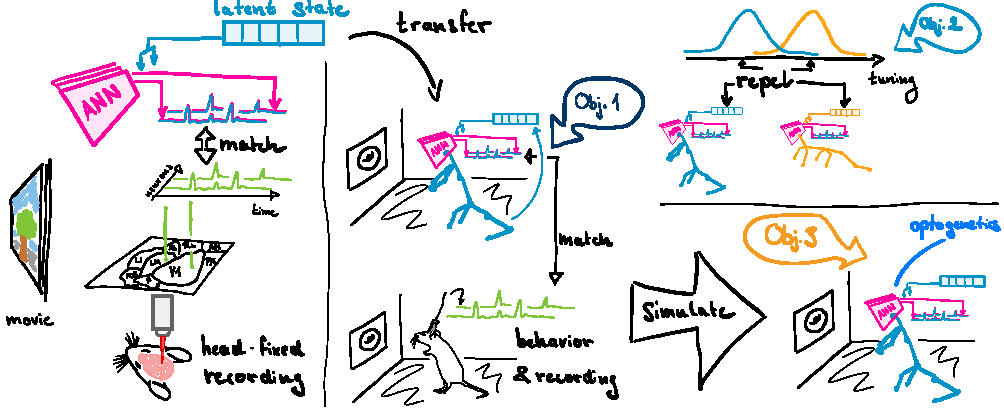
\includegraphics[width=\textwidth, height=7cm]{figures/overview.pdf}
% \end{figure*}

I will build a model for visual cortex under free behavior (\obj{1}), use it to disentangle the contribution of visual input, behavior, and internal state to neuronal activity, and study how behavior and internal state affects neuronal tuning (\obj{2}). Then I will use this model as the visual system in a reinforcement learning agent to predict behavioral strategies of mice in an open field object recognition task. I will use this to study the computational relevance of behavior-associated changes in tuning for task performance (\obj{3}).

If successful, this framework will be a powerful tool to investigate the link between visual representations and behavior, and derive specific predictions about the change of behavior from causal manipulations of the neurons in the visual system.
The framework will not replace experiments, but make it easier, faster and cheaper to generate specific predictions by running experiments \textit{in silico} first before verifying their prediction \textit{in vivo}. 






% -- that allows us to disentangle the contribution of the stimulus, the behavioral context, and internal states to neuronal activity across cortex, to characterize the correspondence between behavioral context and modulation of neuronal processing \textit{in silico}, and that makes testable experimental predictions about neuronal processing that depend on behavioral context or on causal manipulations. 

% Why do we need to consider free/natural behavior?
% - Visual system was made to acquire the information for natural behavior
% - We need natural stimuli, since the visual system might not be as engaged



\subsection{Visual cortex in the context of internal state, and behavior}


% The ultimate question to understand visual representations is \textit{``How does a particular representation serve natural behavior?''}.
Sensory systems provide the informational basis of behavior: Their incomplete and noisy image of environment is our only way to make decisions and pick the next action based on outside up-to-date information. 
At the same time, the brain can choose what to measure: Our actions influence the input to our senses and sensory processing itself adapts to the current behavioral needs. 

The fact that sensory processing changes with motor activity and internal state was first demonstrated by elegant studies on invertebrates many decades ago  \parencite{Rowell1971-zj, Wiersma1968-xt}.
Since then, modulation of sensory responses as a function of behavioral and internal state, such as attention, has been described in many animals \parencite[\eg][]{Maimon2010-sa, Niell2010-bs,Bezdudnaya2006-ge, Treue1996-lp, Musall2019-kd}.
Across animal species, state-dependent modulation predominantly affects neural responsiveness \parencite{Eggermann2014-xp, Niell2010-bs, McAdams1999-cs,Schroder2020-jl, Dadarlat2017-jw, Mineault2016-fk}, resulting in better behavioral performance \parencite{Spitzer1988-kq, Bennett2013-rk, Dadarlat2017-jw, De_Gee2022-ir}.
In a few cases, however, the tuning properties of sensory circuits are also affected by this modulation. 
In the visual system, this has been reported, for instance, for temporal tuning in Drosophila \parencite{Chiappe2010-bm}, rabbits \parencite{Bezdudnaya2006-ge}, and mice \parencite{Andermann2011-vw}, as well as for direction selectivity in primates \parencite{Treue1996-lp}.
Using functional twins based on deep neuronal networks, we recently showed that arousal -- correlated with a dilated pupil and running -- can change the selectivity of neurons in mouse primary visual cortex at the timescale of seconds~\parencite{Franke2022-do}. 
Given that changes in tuning is a widespread phenomenon, I hypothesize that  that there are more ways how neuronal tuning in mouse visual cortex changes with behavior. 
However, a systematic characterization of the correspondence between behavioral context and neuronal function is currently missing. 

Why do visual representations change with behavior? From the perspective of encoding and decoding visual signals, it might seem puzzling to change the encoder because the decoder would need to change, too. 
A likely answer comes from behavior itself:
% However, including behavior can offer a possible explanation: 
When actions need to be chosen on the basis of uncertain sensory information about the world, decreasing this uncertainty about aspects relevant for the current behavioral goal becomes important~\parencite{Chebolu2022-tb}. 
If decreasing uncertainty comes at a cost -- energy or opportunity --, it makes sense to selectively bias visual processing depending on behavioral context, \textit{e.g.} focusing on  higher temporal frequencies during walking, running, and flying periods.
Many known non-visual modulations of neural activity can be understood in that way: 
For instance, when attention increases neural activity in certain neurons, it also selectively increases their signal-to-noise ratio. 
In fact, previous studies reported that modulation of sensory responses resulted in better behavioral performance \parencite{Spitzer1988-kq, Bennett2013-rk, Dadarlat2017-jw, De_Gee2022-ir}.
In these cases, the visual system might bias processing towards visual features relevant for current behavioral goals, such as higher temporal frequencies during walking, running, and flying periods.
However, this means that the change of tuning becomes dependent on the behavioral goal.
Thus characterizing \textit{which} neurons change their tuning, \textit{how} they change it, and under \textit{which behavioral context} will yield useful insights to what end information from these neurons is used under natural conditions.
% This will be the focus of \obj{2}.


Because visual processing might dynamically adapt to behavioral context, we need to characterize neuronal representations under rich variety of behavioral and stimulus contexts to engage the full computational apparatus of the visual system~\parencite{Huk2018-ez, Datta2019-qj}. 
This means we have study how the response of neurons in the visual systems changes in freely behaving (unrestrained) animals using complex naturalistic visual stimuli.
While the vast majority of visual neuroscience still uses head-fixed animals, minimalistic artificial stimuli (such as Gabor patches), and simple tasks (such as 2AFC) there is a trend towards large scale recordings in freely behaving 
 animals~\parencite{Parker2022-ac}.
However, studying neuronal representations and behavior under complex, uncontrolled natural conditions poses new challenges to extract meaningful insights:
% However, this data poses new challenges:
\begin{itemize}
    \item \textbf{Disentangling determinants of neuronal activity:} At any point in time the neuronal activity in the visual system is a result from what the mouse sees (visual stimulus), what it does (motor behavior), and what it wants to do (internal state). 
    To understand how these components shape visual processing, we need to disentangle their contributions to the activity of neurons during free behavior. 
    This includes reconstructing what the animal saw at every moment of the experiment, and developing models that can capture common fluctuations in neuronal population activity.
    \item \textbf{Gaining insights from non-repeatable trials} 
    To characterize how neuronal tuning changes with behavior in a classical experimental trial structure, one would need to present the same stimuli in different behavioral contexts. 
    However, behavior and visual input in natural conditions cannot easily be controlled or repeated, and natural stimuli are not easily parametrized.
\end{itemize}



\subsection{Functional twins: Data-driven models of visual cortex and behavior}
One way to overcome both of the above challenges is to compile many unique behavioral and physiological observations (possibly from multiple experiments) into a single computational model -- a data-driven \textbf{functional twin} -- that allows us to characterize neuronal representations \textit{in silico} and make specific predictions that are testable \textit{in vivo}. 
Functional twins are descriptive models that faithfully predict measurable observations for a real system, such as neural activity or behavior, and extrapolate over a large range of conditions, \textit{e.g.} arbitrary videos or behaviors. 
Thus a functional twin mimics the system \textit{functionally}, without necessarily resembling it \textit{structurally}, like a mechanistic circuit simulation.  

Descriptive models of neuronal function have a long history in systems neuroscience.
Prominent examples include linear nonlinear models of retinal ganglion cells~\parencite{Paninski2004-ax,Pillow2008-me}, quadratic energy models of complex cells~\parencite{Adelson1985-re}, divisive normalization models to account for complex contextual modulations~\parencite{Heeger1992-xx}, or subunit/LN-LN models~\parencite{Rust2005-ro,Touryan2005-pi,Vintch2015-gc}.
While these models did not consist of biophysically meaningful components, they still had a low number of interpretable parameters, such as a linear filter. 
However, while these models yielded good predictions for earlier stages of the visual system or particular stimulus subspaces (like Gabors or gratings), their structure was still hand-crafted and too constrained \hl{double check Gallant}. 
One consequence of that was that they did not generalize well across different stimuli, such as natural images, and were too constrained to reflect the complexities of neurons in higher visual areas or species other than cat or monkey, which inspired these models.
One avenue of research to address that problem turned to more flexible multi-layer neural networks with more parameters~\parencite{Zipser1988-nh,Lehky1992-wf,Lau2002-gb,Prenger2004-qu}.
The advent of deep learning also led to tremendous progress in this area of model building for neuroscience: task-optimized deep convolutional neural networks (CNNs) \parencite{Yamins2014-cg,Cadieu2014-gc,Cadena2017-rb} and CNN-based architectures learned end-to-end on physiological recordings set new standards in the prediction quality and extrapolation capability~\parencite{Antolik2016-va,Batty2016-do,McIntosh2016-tr,Klindt2017-sb,Kindel2017-xs,Cadena2017-rb,Burg2021-yg, Lurz2020-ua, Bashiri2021-or,Zhang2018-cs,Cowley2020-cy,Ecker2018-gz, Sinz2018-sk, Walker2019-yw, Franke2022-do}. 


The use of models trained end-to-end on data from physiological experiments marks a paradigm shift from models with easily interpretable parameters to large models whose major goal is to mimic the neuronal system as closely as possible so that parts that are experimentally difficult, such as \eg search for optimal stimuli, can be outsourced to an \textit{in silico} experiment in the model. 
The authors of the \textit{neuroconnectionist research programme}~\parencite{Doerig2022-ex} advocated a ``large-scale research programme centered around ANNs as a computational language for expressing falsifiable theories about brain computation'' that generate ``new and otherwise unreachable insights into the workings of the brain''. 
Importantly, however, the results of the \textit{in silico} experiment are usually easier to verify \textit{in vivo}. 
For instance, search optimal for unconstrained images that strongly excite neuron is next to impossible in experiments, since search space is enormous, but feasible in the model using optimization.
The stimulating properties of the resulting image, however, can be efficiently verified in follow-up experiments~\parencite{Walker2019-yw}.
To emphasize this intention, we call these models \textit{functional twins}. 
The unrealized potential of this approach to integrate complex experimental data, generate new predictions, and speed up our understanding of the brain is enormous. 

\begin{figure*}[t]
    \centering
    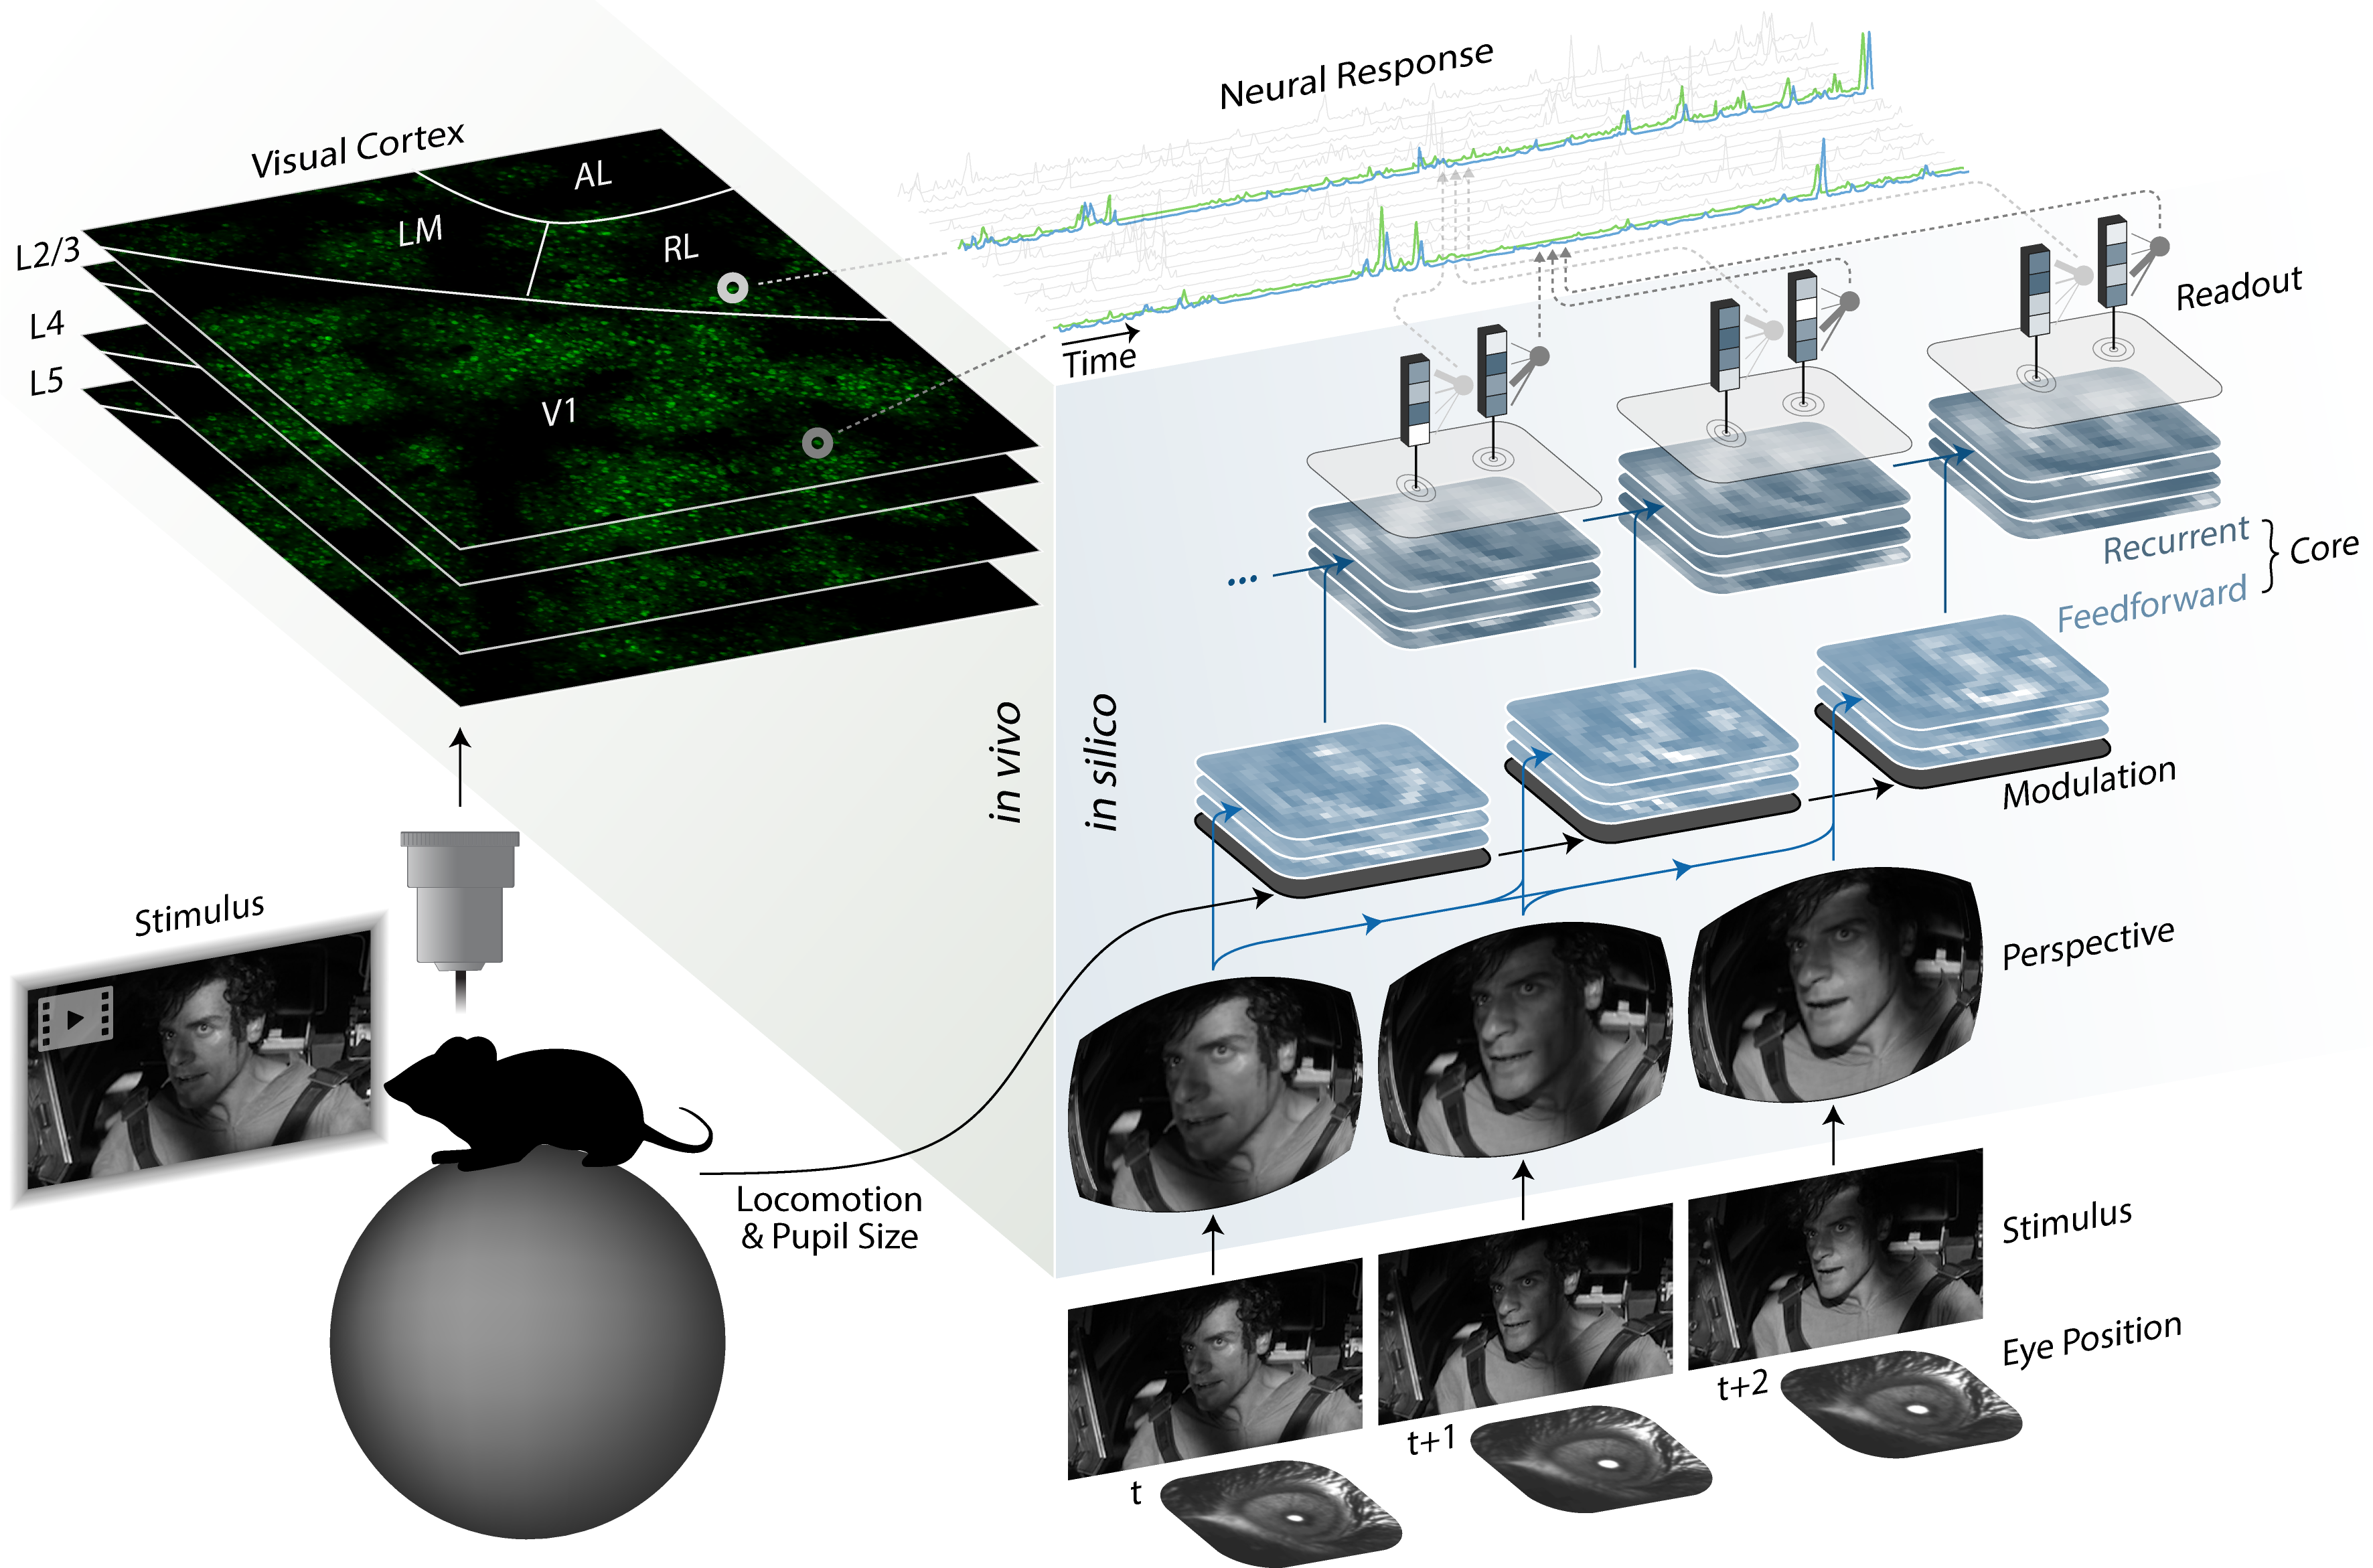
\includegraphics[width=.9\textwidth]{figures/architecure_v9.png}
    \caption{Schematic from Eric: Replace}
    \label{fig:videomodel}
\end{figure*}

My group and I made substantial contributions to the development of data-driven models, trained end-to-end on neuronal responses and natural images or video~\parencite{Sinz2018-sk, Walker2019-yw, Lurz2020-ua, Bashiri2021-or, Lurz2022-up, Franke2022-do, Cobos2022-rr, Ecker2018-gz,Cadena2019-jw}. 
I developed the first deep model primary visual cortex on natural video~\parencite{Sinz2018-sk}, which was also the first model to include simple forms of behavioral variables, such as running speed or pupil dilation, and the first to incorporate gaze prediction of the animal as part of an end-to-end trained model (see Fig.~\ref{fig:videomodel}). 
We were the first to combine fully image driven model with latent state models that capture common fluctuations caused by internal states~\parencite{Bashiri2021-or}.
In addition, we can infer boundaries between brain areas just from recordings of natural images, something that usually requires additional experiments~\parencite{Bashiri2021-or}.
We also demonstrated that these models learn characteristic feature representations for visual cortex that generalize well between neurons and animals~\parencite{Lurz2020-ua,Cobos2022-rr}.
Models based on our network architectures are currently state of the art in predicting mouse visual cortex\footnote{All winners of  \url{https://sensorium2022.net/} used our base network architecture}. 
Furthermore, we~\parencite{Walker2019-yw} developed the \textit{inception loops} paradigm that uses data-driven models of the visual system to synthesized new optimal stimuli for specific neurons that can readily be verified in follow-up experiments\footnote{Other groups from Harvard~\parencite{Ponce2019-yn} and MIT~\parencite{Bashivan2019-ry} concurrently published similar techniques for monkey visual cortex.}. 
Using this technique, we demonstrated that optimal stimuli for mouse primary visual cortex substantially deviated from previous text book models of visual tuning~\parencite{Hubel1959-zs}, and that selectivity of these neurons can change with arousal on the order of seconds~\parencite{Franke2022-do}.
Other labs are using our models to gather new insights about the visual system~\parencite{Hofling2022-wr} or model it under complex conditions~\parencite{Parker2022-ac}.

This modeling approach is a great step forward as it allows neuroscience researchers to model passively viewing experiment. 
However, the visual system is not a passive observer and many neuroscience experiments involve a task or behavior to understand causal effects of the visual representations onto the actions of an animal. 
Since, behavioral experiments are tedious and time consuming, and since it is hard to make predictions for natural behavior, a modeling approach that integrates neuronal activity and flexible behavior would be very beneficial for neuroscience. 
However, several keys steps for such a model are missing. 
To model the effect of behavior on visual processing, we need a model that can capture this effect. 
Since the number of simultaneously recordable neurons in freely behaving animals is still orders of magnitude lower than in head-fixed animals, training such a model from scratch on one experiment only likely would not realize the full predictive power of such a model. 
Thus, we need effective transfer learning schemes to pre-train a model on head-fixed data and transfer it to freely behaving animals in a way that still allows us to capture how behavior influences visual processing. 
To model visual cortex under free viewing, we need to know the visual input to the mouse. 
This means we need to track experimentally its gaze, which is technically challenging, or we need to infer the gaze from video recordings of the animal and simultaneous recordings of neuronal activity. 
Furthermore, if we want to make predictions about how visual system about behavior, we need to provide the possibility for the model to behave differently than what we observed (to answer ``what if'' type of questions). 
This means we have to be able to predict the visual input from new viewpoints.
Existing approaches that put a camera on top of a mouse~\parencite{Parker2022-ac} do not allow for that. 
Other approaches that used a digitized environment, did not model neuronal activity~\parencite{Holmgren2021-jv}.
Finally, there is no previous work that combines a model of a real neuronal visual system with a model that selects actions of a mouse in free behavior. 
This is needed, however, to make predictions about how neuronal visual processing mechanisms affect behavior. 

% modeling a visual system of a free running mouse that captures the effect of  during free behavior that captures the interaction requires a 
% \hl{What's the gap: Behavior and video. Latent states. Interaction between the two. }
% \hl{Simulation of different behavioral input}
% \hl{For behavior: What if the mouse did something else -> visual input changes  }

\subsection{Studying the effect of visual representations on behavior}
% virtual mouse, the paper by the guy from Freiburg, Deepmind paper, some Dayan work maybe?
The gold-standard in understanding the computational role of visual representations is to quantify how causal manipulations of it affect behavior. 
For instance, if behavior-associated changes in neuronal tuning serve to decrease uncertainty in relevant world dimensions, then turning off these changes through causal manipulations of the neuronal circuit should result in a higher variance or lower accuracy of the animal's performance in a task, or in some kind of compensatory behavior, such as longer decision times.
These kinds of questions pose many experimental challenges. 
The first is to come up with a specific prediction for the behavioral effect of the causal manipulation: For instance, other neuronal circuits parallel or downstream of the manipulation might have complex effects on the decision of the behavior of an animal that can be hard to control. 
Second, to experimentally show the effect, animals need to be trained on a task which is time consuming and tedious. 
A computational model that uses a function twin of the visual system and that can make specific behavioral predictions, and thus be used to pre-screen possible tasks and predictions, would tremendously speed up neuroscience research in this regard. 
Here, I propose to take an important step in this direction. 

To answer causal questions about visual representations we need components that involves a task structure (\eg specified by a reward) and derives behavior from that. 
This is the domain of reinforcement learning.
There is a large literature that studies the neuronal basis of decisions and motor behavior of animals using reinforcement learning, imitation learning, or optimal control~\parencite{Schultz1997-xu}\hl{more refs}.
Recently, \parencite{Kalweit2022-ev} showed that accounting for the intrinsic reward inferred via inverse reinforcement learning, they can improve the predicted accuracy of a mouse's behavior by approximately 40\%.
However, all previous studies either assume that the state of the environment is know to the animal, use strongly simplified (low dimensional) sensory models, or study a very constrained environment with a severely limited action space. 

On the other hand, the it has been demonstrated in the recent past that combining reinforcement learning or imitation learning algorithms with deep network based vision models is feasible. 
\textcite{Merel2020-hf} trained a virtual rat to perform tasks in a virtual environment and studied the representations in the learned visual system of the agent onto task behavior and demonstrated that they could obtain meaningful results with ablating selected neurons in the circuit. 
\textcite{Deverett2019-gs} explored the effect of recurrence in an artificial neural network on behavior. 
The show that the ablation of recurrent connections removes the agents ability to internally measure time and that the agent uses behavior to measure time instead. 
Interestingly, measuring time by rythmic motor behavior has been studied in animals behavior and known as stigmergy.
Furthermore, \textcite{Hilton2020-jz} showed that altering the image feature extractor model or a reinforcement learning agent results in predictable changes of behavior.
While all of these machine learning studies demonstrate that the effect of altering the ``visual system'' of a virtual agent on behavior can be systematically studied, none of these studies use neuronal data, realistic models of a visual system, or real behavior of animals. 
A computational framework that integrates large scale neuronal activity in the visual system and behavior in a realistic environment or task, is currently non-existent. 
The mouse is an almost perfect model system for this. 
The absence of a fovea and the relatively low resolution of the visual system, makes it easier to model its visual system, and the genetic toolbox available offer many opportunities to test the effect of causal manipulations onto behavior \textit{in vivo}.

\subsection{Objectives}
I propose to characterize changes in neuronal tuning under spontaneous and goal-driven behavior using data-driven functional twins of mouse visual cortex merged with detailed behavior described by skeleton graphs in digitized environments.
% such that changes of visual computations with behavior and internal state are preserved. 
Furthermore, I propose to develop a computational framework based on the model and reinforcement learning to make causal predictions about the behavioral relevance of these mechanisms. The project has three objectives (click on \obj{1}, \obj{2}, \obj{3}):
% The scientific questions laid out above, all require substantial methodological innovations in machine learning for neuroscience, and can be broken into three objectives.
% . Thus each objective has a technical goal and a scientific question. 

% \subsubsection{Objectives}
% \subsubsection{Objectives}
\begin{itemize}[leftmargin=2em,topsep=0pt,itemsep=0.62ex,partopsep=0ex,parsep=0.5ex,rightmargin=1ex]
    \item[\obj{1}] \textbf{Disambiguate the contributions of stimulus, behavior, and internal state} to neuronal responses in miniscope recordings of freely behaving mice  by developing \textbf{a video-driven functional twin of mouse visual cortex and motor behavior} in digitized real environments. This model will form the backbone for \obj{2} and \obj{3}. 
    \item[\obj{2}] \textbf{Characterize behavior-associated changes in neuronal tuning} and how they relate to
    uncertainty about properties of a scene. To this end, we will learn a low-dimensional behavioral embedding for tracked behavior, find directions in that embedding space that maximally change neuronal tuning, and decode scene properties from the model under the different tuning extremes. I expect to find changes in tuning that differ across brain areas and are linked to decreasing  uncertainty about specific scene properties for defined behavioral contexts. 
    \item[\obj{3}] \textbf{Characterize relevance of tuning changes for goal-driven behavior} by building a computational framework based on the functional twin and reinforcement/imitation learning to predict the effect of tuning changes onto behavior. We will validate the framework with data from experiments with optogenetic manipulation of visual cortex. I expect that en- and disabling tuning changes in the model mostly affects behavior/performance in tasks that involve motifs associated with the tuning change, as identified in \obj{2}.
% The framework will yield experimentally testable predictions about the effect of causal manipulation of the neuronal population or the stimulus on behavior. 
\end{itemize}

\subsection{Significance}
% \subsubsection{Interdisciplinarity}

\textbf{Interdisciplinarity} This project develops novel machine learning methods for fundamental research questions in neuroscience, and requires strong expertise in both fields. 
I am trained in bioinformatics (undergraduate), machine learning (since undergraduate), computational neuroscience (PhD), and neuroscience (PostDocs). 
I was the coordinator for machine learning and computational neuroscience in a large consortium\footnote{Machine Intelligence from Cortical Networks: \url{https://ninai.org}} to understand the cortical algorithms of vision.
% that recorded the visual responses and circuit anatomy of about 60,000 neurons to natural, parametric, and rendered movies. 
This and multiple follow-up projects gives me access to \hl{several million neuron hours} of responses to natural videos across the entire visual cortex. In addition, my long-time collaborators Dr. Tolias (Baylor College of Medicine, Houston, co-authors on >20  publications) and Dr. Froudarakis (FORTH, Crete, co-authors on >10 publications) will provide me with physiological and behavioral data from freely behaving mice. 


\textbf{Beyond state of the art \& potential impact} 
The proposed project develops crucial computational technology to step away from the typical trial based structure of systems and behavioral neuroscience towards a ``natural neuroscience'' that focuses on studying a neural system under complex natural conditions that cannot easily controlled or repeated. 
If successful, it can change our view on visual cortex in mice and how neuronal tuning is changed according to behavioral needs. 
% Even in classical conditions every trial in a neuronal system depends on uncontrollable factors (e.g. internal state) and can thus not be exactly repeated~\parencite{Urai2022-fz}. 
% I advocate to embrace this complexity and build models that can compile many experiments in a single model, can disentangle different factors of neuronal processing, yet make specific and verifiable experimental predictions. 
It pushes multiple boundaries of model development in neuronal data science with many applications beyond this project. \circled[black][black][white]{1} Most current models for visual cortex focus on static images, are built for head-fixed animals, and only account for very impoverished behavioral variables (such as running vs. not-running, or pupil dilation). The video-based latent-state model from \obj{1} embedded into digitized environments thus takes several steps forward and merges two major determinants of a neuronal system: stimulus driven neuronal activity and behavior. It is straightforward to generalize to include other areas (such as motor or prefrontal areas), or stimulus modalities (such as olfaction or sound), or more detailed observations (such as whisking or biophysical body models). 
\circled[black][black][white]{2} The use of reinforcement learning in combination with functional twins of visual cortex and causal manipulations (\obj{3}) is unprecedented, and offers an innovative way to bridge the gap between visual representations and behavior. The framework is readily generalizable to other tasks and questions and will be a powerful tool to investigate the link between sensory representations and behavior, and derive specific predictions about the change of behavior from causal manipulations of the neurons in the visual system.
\circled[black][black][white]{3} Together they allow a comprehensive characterization of how the visual system adapts with behavioral context. As the volume, detail, and complexity of neuroscientific and behavioral data is increasing, the proposed approach is one step towards a \textit{standard model of systems neuroscience}.
The framework will not replace experiments, but make it easier, faster and cheaper to generate specific predictions by running experiments \textit{in silico} first before verifying their prediction \textit{in vivo}.

\textbf{Ethics in AI and the use of animals}
The misuse of machine learning can negatively impact the lives of individuals with respect to privacy, discrimination or bias. 
My proposed project is about developing computational tools for fundamental research in systems and behavioral neuroscience. 
Thus, there are no foreseeable direct negative consequences on the life of individuals and it is unlikely that my research will result in negative consequences regarding ethical concerns related to human rights and values.

Although, we study neuronal systems and use large scale neuronal data, my lab will not perform any animal experiments in this project. 
The experiments for a large fraction of the data volume that we want to use for this project have already been recorded. 
In addition, I have included a small budget for subcontracting supplementary experiments at the labs of my experimental partners Emmanouil Froudarakis (FORTH, Crete) and Andreas Tolias (Baylor College of Medicine, Houston, Texas).  
While the success of the project does not depend on these experiments, experimental verification of our predictions will make our results more impactful. 
They will be carried out in agreement with ethical regulations and protocols approved by \hl{Manolis FORTH} and Baylor College of Medicine Institutional Animal Care and Use Committee (IACUC).
%%%%%%%%%%%%% METHODOLOGY %%%%%%%%%%%%%%%%%%%
\section{Methodology}
% \subsection{A data-driven embodied digital twin of mouse visual cortex}
% % \subsection{\color{obj1}Objective 1: A data-driven embodied digital twin of mouse visual cortex}
\subsection{\colorbox{obj1}{\color{white}Objective 1}: \oonetitle}
\labelobj{1}

\textbf{Overview and rationale:} Neural activity and tuning in visual cortex is not only determined by visual input, but can be profoundly affected by behavior and the internal state of an animal~\parencite{Niell2010-bs,Musall2019-kd,Stringer2019-lt, Franke2022-do}.
To link the computations in the visual system to behavior and understand the interactions between the two, we need to see as much of the visual system ``in action'' as possible. 
While it is now possible to record hundreds of neurons during free behavior~\parencite{Parker2022-ac}, we are still not at the scale in terms of the number of neurons that can be reached with 2-photon. 
Here, I propose to use deep learning to pre-train a video-based model of tens of thousands of excitatory neurons from multiple areas of the visual system on visual responses recorded with 2-photon from head-fixed mice, and put it ``into the mouse's shoes'' by fitting it to recordings from a miniscope attached to a tracked stick-figure model of a freely behaving mouse in a  digitized version of its environment.
We will endow this model with an unobserved latent state that can capture variability due to non-visual signals~\parencite{Musall2019-kd, Bashiri2021-or}.
When we attach the large scale model to the mouse in the digitized environment we will use the fewer neurons from the miniscope to infer the exact eye movements of the mouse and explain non-visual neuronal variability from the actual behavior of the mouse and the internal state inferred from the population activity.
This approach offers several benefits
\begin{enumerate}[topsep=0pt,itemsep=0.62ex,partopsep=0ex,parsep=0.5ex]
    \item We previously showed that models pre-trained on many recordings can be fit more efficiently to new neurons and stimuli using transfer learning~\parencite{Lurz2020-ua}. We thus expect a better predictive power than when directly fitting a model to a few hundred neurons recorded during free behavior. 
    \item Since previous work has found the non-visual fluctuations to be relatively low dimensional, we can identify the relevant dimensions in the head-fixed recordings first, and use the fewer neurons recorded with the miniscope to infer the actual state $\vec{z}$ of the fluctuations in the lower dimensional space. We can then explain fluctuations in $\vec{z}$ via the actual behavior and thus disentangle the contributions of visual input, behavioral state, and internal state to neuronal activity. 
    \item In addition, by feeding the visual input from the tracked mouse and the inferred latent state $\vec{z}$ back to the model, we can predict the activity of all neurons from the head-fixed recordings as if they were attached to the mouse and shared the same brain state.
    \item The model in the digitized environment allows us to simulate neuronal activity in new situations that have not been observed in the data (\objii) and even use the model as a virtual agent to simulate task driven behavior (\objiii).
\end{enumerate}

The objective is split into three work packages. 
Building on my previous work~\parencite{Sinz2018-sk, Bashiri2021-or}, \objwp{1}{1} develops a video-driven latent state functional digital twin model. 
The technical innovation is to include a latent state into a dynamic model that can accurately capture low-dimensional population dynamics from non-visual sources, and can easily be adapted to new neurons and mice. 
\objwp{1}{2} builds the embodied digital twin by first building a digitized model of the environment of the mouse and inferring the 3D trajectories of the animal's pose from video data, and then attaching the model from \objwp{1}{1} to the mouse predicted eye positions and fine-tuning it to  miniscope recordings of a few hundred neurons from different visual areas, inferring the eye positions and brain state using the recordings. 

\textbf{Scientific goal:} This model will allow us to disentangle the contributions of visual input, behavior, and internal state to neuronal activity in visual cortex during free behavior, and investigate my hypothesis that behavior influences each higher visual area in different ways. \hl{possibly adapt hypothesis}

\textbf{Technical innovation:} This will be the first encoding model that predicts the activity of tens of thousands of neurons in visual cortex under free behavior and accounts for the modulation of neurons from brain state and behavior -- yielding an embodied functional digital twin that can be used to simulate new situations as close to real activity as currently possible.



\subsubsection{Work package 1.1: A video-driven latent state model of the visual system\hfill\objwp{1}{2}}
\labelobjwp{1}{1}
\hl{Add equations}
% We will pre-train a model for visual responses on many thousands of neural responses across visual cortex from head-fixed mice presented with video. 
Like in my previous work, the model will consist of a \textit{common feature extractor} that extracts nonlinear features for each brain area from a given video using 3D convolutional and recurrent deep networks.
We will turn the model into a latent variable model by adding a Gaussian latent state to this feature representation and use linear \textit{readout mechanisms} to predict neuronal responses transformed with a neuron-wise non-linear flow transformation~\parencite{Bashiri2021-or, Rezende2015-mx}.
Since neural response have at least one discrete component, we will use variational dequantization to first turn the discrete component into a continuous one~\parencite{Hoogeboom2021-zs}.
Correlations between neurons will be modeled by allowing the latent state to be correlated across space and time. 
In the image based model~\parencite{Bashiri2021-or}, we used a factor analysis model. 
For the dynamic model, we will either extend the factor analyzer to a finite window in time, or use a linear Gauss-Markov model (generative model of a Kalman filter) to stay efficient. 
As before, we will integrate over the latent state for fitting and train the model on the marginal likelihood of the transformed neural responses given the video.
Because of the variational dequantization (but not the latent state), we need to use variational inference to train the model on the marginal likelihood. 
% If necessary, we can also let the correlation structure depend on the visual input. 
\hl{include what data the model is trained on, do we include behavioral state, or just compare to it.}

\subsubsection{Work package 1.2: Embodied digital twin\hfill\objwp{1}{2}}
\labelobjwp{1}{2}

\textbf{Behavior via posture graph trajectories}
We will track the movement of the mouse in the cage from one or more cameras \hl{be speciic}, and detect 2D keypoints of its posture graph using DeepLabCut~\parencite{Mathis2018-lk}. 
Subsequently, we will lift this 2D graph to a 3D posture graph using our pose lifting model~\parencite{Pierzchlewicz2022-tq}. 
For freely moving humans, this model achieves an accuracy of less than 5mm and can also deal with temporarily occluded keypoints. 
This step will yield a 3D trajectory of a stick-figure model of the mouse in its environment over time. 

\textbf{Digitize environment:} 
We will build a virtual model of the environment using LIDAR and baking images of the animal's cage as texture onto the scanned mesh~\parencite[similar as in][]{Holmgren2021-jv}.
This is established technology can theoretically be done with an iPhone Pro 12, although we will purchase a more high-end solution.
Subsequently, we will use Blender and PyTorch to move our model in the environment according to the movement of the mouse from.
Since the cage and lab environment are standardized and static, we can do that for the existing data in hindsight.

\textbf{Embodied digital twin:} We will place the model learned from \objwp{1}{1} at the approximate eye locations of the mouse inferred from tracking the mouse and move it in the digitized environment according to the movement of the mouse. 
We will additionally account for the fact that mice do compensatory eye movements during locomotion\hl{REF} to get as close as possible to the true gaze position. 
We will then fine-tune the gaze position in each frame by optimizing the exact locations along with the linear readout components for the recorded neurons. 
The fact that all neurons are affected by the gaze direction in the same way, makes it possible to identify the parameters from gaze as already demonstrated by similar approaches of us and others before~\parencite{Sinz2018-sk,Walker2019-yw,Parker2022-ac}.
We will then include the posture trajectory of the animal as an additional input to the model to explain as much of the latent state as possible. 

\subsubsection{Expected outcome} 

An embodied functional digital twin of the visual system of the mouse that allows us to disentangle the contributions of visual input, behavior, and internal state to neuron activity during free behavior. 
Importantly, it will allow us to predict neuronal activity to completely novel trajectories of the mouse in the environment.

\hl{How will we test/analyze the model}
% Using this model we will the cluster neurons depending on how they are affected by behavior and internal state.
% We expect that neurons co-cluster with areas, i.e. that neurons in different areas are differently affected by behavior. 

\subsubsection{Risk management} 
\hl{What if we cannot estimate the eye position from neural data?}
\hl{What about modulations from other modalities (non-visual cues)?}
\hl{Digital twin of 1 not binocular. How to deal with that?}

%%%%%%%%%%%%%%%%%%%%%%%%%%%%%%%%%%%%%%%%%%%%%%%%%%%%%%%%%%%%%%%%%%%%%%%%%%%%%%
\subsection{\colorbox{obj2}{\color{white}Objective 2}: \otwotitle.}
% \subsection{\color{obj2} Objective 2: Find tuning changes and characterize uncertainty in latent dimensions.}

\label{sub:obj2}

\textbf{Overview and rationale:} 
\hl{Different brain areas in?}
Behavior and state of arousal can modulate the response of neurons in mouse visual cortex~\parencite{Niell2010-bs, Stringer2019-lt, Musall2019-kd}.
We have recently demonstrated that tuning of neurons to color in mouse V1 can change with the behavioral state of the animal~\parencite{Franke2022-do}.
Whether this finding is only a single instance or whether there is a larger spectrum of tuning change with behavioral state is currently an open question. 
However, given that many motor behaviors can be described within the framework of stochastic optimal control~\parencite{Todorov2004-yb}, and that the dual objective of a good controller is to (i) achieve the desired target and (ii) reduce uncertainty about the state~\parencite{Patchell1971-zk}, it is likely that there are other changes of neural representation in visual cortex that serve to reduce the uncertainty about the state of the animal. 
In fact, existing changes already reduce uncertainty as a change in gain -- usually correlated with running or arousal -- increases the signal to noise ratio in sensory neurons. 
This objective investigates this idea by searching for sets of behavioral motifs that maximally change tuning of given neurons (\objwp{2}{1}) and relating these changes to the change in certainty about different stimulus aspects obtained from rendered stimuli by decoding them from neuronal responses using the embodied digital twin model (\objwp{2}{2}).




% The detailed movement of the posture graph of each animal in 3D, although constrainted by the biophysical movement apparatus of the mouse, likely contains more details and is too high-dimensional to extract meaningful stereotypical behaviors that can be related to modulation of neuronal activity. 
% Even though automated tracking of animals has made huge steps forward with tools such as DeepLabCut~\parencite{Mathis2018-lk, Schneider2022-qf}, automatic and unsupervised clustering into discrete units is still an open problem. 
% In this objective we will use methods from unsupervised probabilistic machine learning to embed bouts of 3D posture trajectories from \obji~into a low dimensional space and cluster them into single actions or tokens. 
% We will then use this low-dimensional representations to relate the modulation of neurons in the model of~\obji~to stereotypical behaviors. 
% The tokens will also play a key role in the reinforcement learning model in objective~\objiii.

\textbf{Scientific goals:} What stereotypical behaviors change the tuning of cells in different areas the most? How doe these changes relate to certainty about different latent stimulus dimensions?

% \textbf{Technical innovation:} 
% An unsupervised generative model to tokenize free behavior of mice into single actions, generate novel smooth behavioral trajectories, and automatically extract an ethogram of behavior.


\subsubsection{Workpackage 2.1\hfill \objwp{2}{1}}
\labelobjwp{2}{1}
The detailed movement of the posture graph of each animal in 3D, although constrained by the biophysical movement apparatus of the mouse, likely contains more details and is too high-dimensional to extract meaningful stereotypical behaviors that can be related to modulation of neuronal activity. 
To find behavioral motifs from the 3D trajectories of the postures, we will first fit a latent state probabilistic model to the trajectories that describe the in terms of a low dimensional continuous latent state and a clustering of those embedding into discrete motifs.
To that end, we will train a variational autoencoder (VAE) similar to the hidden Markov model proposed by the MoSeq toolbox~\parencite{Wiltschko2015-ey, Wiltschko2020-zd} on the 3D graphs from~\objwp{1}{2}.
Since this model can generate 3D graphs, we will connect it the model of~\objwp{1}{1} to obtain a model in terms of stimulus and latent behavioral embedding
\begin{center}
    \texttt{neural responses = model(video stimulus, 3D postures(embedding))}.
\end{center}
Note that the video stimulus would usually be a function of the 3D postures and eye movements, since this determines where the animal looks in the world. 
However, using our digital twin model, we can decouple the stimulus from the behavior and use it to find pairs of stimuli and embeddings (and their corresponding 3D posture) describe tuning changes of single neurons with respect to behavior. 
To this end, we will find directions in the behavior embedding space that maximally modulate the response of a given neuron to the same stimulus, i.e. change its tuning.
This can be done using optimization on the embedding space. 
To not overfit to spurious directions, we will jointly optimize such a direction for many stimuli that elicit a response in  a given neuron at once. 
To visualize the changes in tuning, we will compute maximally exciting input~\parencite[MEIs][]{Walker2019-yw} for each extreme of the behaviors found in embedding space. 
\hl{add rendering}

\subsubsection{Workpackage 2.2\hfill \objwp{2}{2}}
\labelobjwp{2}{2}
If the tuning change has influence on behavior and the decision of the animal, then natural occurring variations in the neuronal responses should have an influence on the task performance of the mouse. 
We will thus use the behavioral embedding or, alternatively, the latent state inferred by the model from the neuronal responses, and compute choice correlation to determine whether behavior or tuning changes are informative about the choice, and thus the task performance of the animal. 
In particular, we will analyze whether either the behavior or the latent state differ between trials where the animal made the correct decision vs. trials when it decided wrong. 


\subsubsection{Workpackage 2.3\hfill \objwp{2}{3}}
\labelobjwp{2}{3}

One of the objectives of stochastic optimal control is to reduce the uncertainty about the state determined (among others senses) by the visual system. 
Since not every aspect of the environment is equally important for every behavior, we hypothesize that tuning changes corresponding do different behavioral motifs found in~\objwp{2}{1} also affect the certainty about different stimulus dimensions. 
To investigate this, we will decode latent world properties, such as object boundaries, depth, curvature, slant, texture, and optical flow, that are available to us from rendered stimuli from neuronal responses\hl{where do we have them from; model only or head-fixed; or otherwise?} under the different tunings of the neural population corresponding to different behavioral motifs identified in~\objwp{2}{1}.
To that end, we will train another convolutional or recurrent core of the network from~\objwp{1}{1} to reproduce the features of the original core by minimizing
\begin{center}
    \texttt{$\|$original\_core(rendered video) - new\_core(world properties)$\|^2$}
\end{center}
with respect to the parameters (network weights) of \texttt{new\_core}. 
Note, that this does not require neural responses rendered stimuli, only pairs of rendered videos and latent dimensions, which are cheap to generate. 
We have previously demonstrated that matching the outputs of a core can reproduce the essential features for neural prediction~\parencite{Safarani2021-yy}.
This yields a new model 
\begin{center}
    \texttt{neural responses = model(world properties, 3D postures(embedding))}.
\end{center}
We will test this model with trials from experiments where a mouse was presented with rendered movies \hl{mention where we have them from}. 
We can then decode the world properties from neural responses by optimizing them to match the real neuronal response using the model and different behavioral motifs.\hl{find better name} 
We have previously demonstrated with models for static natural images and verification experiments~\parencite{Cobos2022-rr}, that this approach best captures the perceptual relevant dimensions for mouse visual cortex. 
We will then quantify the accuracy and variability with which different world properties are decoded under different behavioral states. 

\subsubsection{Expected outcome} 
I expect the change in tuning to change the certainty and accuracy in specific behaviorally relevant world dimensions. 
For example, figure ground segmentation could increase the upper visual field when the animal is alert~\parencite[similar to findings in ][]{Franke2022-do}.
Other possible changes could be that neurons become more invariant to optic flow generated by the own movement of the animal \hl{how would we exactly find that?}, that optic flow is better decoded during still periods to detect approaching objects when the animal is an easy target, or that object borders are boosted during locomotion for better landmark detection. 

\subsubsection{Risk management} 
\hl{TODO}
%-------------------------------------------------------------------------------------



%%%%%%%%%%%%%%%%%%%%%%%%%%%%%%%%%%%%%%%%%%%%%%%%%%%%%%%%%%%%%%%%%%%%%%%%%%%%%%
\subsection{\colorbox{obj3}{\color{white}Objective 3}: \othreetitle .}
\label{sub:obj3}

\textbf{Overview and rationale:} 
Previous studies reported that modulation of sensory responses resulted in better behavioral performance \parencite{Spitzer1988-kq, Bennett2013-rk, Dadarlat2017-jw, De_Gee2022-ir}.
I thus hypothesize that tuning changes in general bias visual processing towards task- or behavioral relevant signals.
\obj{2} identified how changes in tuning \textit{correlate} with behavior.
However, to determine whether these changes are relevant for downstream mechanisms to determine behavior, we need to establish \textit{necessity}. 
The goal of this objective is to build a computational framework to predict how behavior and task performance of an animal would change if its visual system did not exhibit behavior-associated changes in tuning. 
This a challenging causal and counterfactual question.
To difficulty for making such a prediction for free (open field) behavior results from the redundancy or the visual stimulus or the representation in the visual sytem. 
Even when a particular neural mechanism is suppressed or altered, there might be other ways for the animal to still achieve the behavioral goal. 
As a consequence, the behavioral changes might be subtle and thus hard to predict or interpret.
We will thus build a to the computational framework in several steps. 
We will first capture the effect of optogenetic manipulations one the neuronal representations in the model using large scale recordings from head-fixed animals. 
We will then model the effect of these manipulations on the decisions of the mouse in a object recognition task during head-fixed and open field behavior. 
Since, we will have the corresponding experimental data, this will be a strong test whether our model can indeed capture the effect of causal manipulations on behavior.
Once that is established, we will use this framework to model how the open field behavior will be affected if we turn-off behavior-associated changes in tuning.
% The goal of this objective is to build a computational framework to predict how changes in tuning affect goal-driven behavior and task performance of an animal in an open field object recognition task. 
% , the experimental intervention must be massive to block the entire flow of information, or the behavioral paradigm needs to be very elaborate to exclude other sources of information. 
% All of that is tedious, expensive, and time consuming. 
To model the effect of changes in visual representations on behavior in open field behavior, we need to account for the possibility that the animal chooses a different strategy to still solve the same task. 
This means, we need to allow our model to change its behavior to solve the task. 
To that end, I propose use the functional twin of in combination with imitation or reinforcement learning.
The reinforcement learning agent will have the previously learned visual system of a mouse (with and without manipulations) to access the state of the environment.
The learned behavioral policy of the agent will make predictions about the behavior of the animal. 
When the manipulation is turned on, the agent can either use the previously learned policy or adapt the policy to compensate for the changes in the visual system.
Both will make a prediction about the change in behavior of the animal. 

\textbf{Scientific goals:}  Predict whether behavior-associated changes in visual representation 
are necessary to predict the behavior and performance of an animal. 

\textbf{Technical innovation:} 
Build a computational framework based on imitation and reinforcement learning to predict the causal effect of changes in the neuronal representation on behavior. 
% An unsupervised generative model to tokenize free behavior of mice into single actions, generate novel smooth behavioral trajectories, and automatically extract an ethogram of behavior.

\subsubsection{Workpackage 3.1: Causal manipulations in head-fixed animals\hfill\objwp{3}{1}}
\labelobjwp{3}{1}
We will model the effect of optogenetic inhibition of different areas onto decisions of mice in two alternative forced choice object recognition task. 
The data consists of large-scale recordings from multiple visual areas in different mice performing the object recognition task under normal conditions and when particular areas are optogenetically suppressed\hl{which areas?}.
We will first model whether we can predict the animals decisions under normal conditions. 
To that end, we will train a model to predict the correct outcome for each trial from the feature representation of the functional twin (from the core) just using the mean latent state of the model.
We will then freeze the task decoder and enable the latent state in the visual model. 
We will infer the latent state from the actual neuronal recordings.
Then we will compare the decisions of the model with the decisions of the animal. 
We expect that addition the latent state increase the prediction accuracy of the choices of the animal. 

In the next step, we will extend the model to account for the effect of opto-genetic manipulations. 
To that end, we will include an additional input to the model that indicates whether the manipulation was on or off. 
We will freeze the readout of the actually predicted neurons and then only adapt the feature representations (core) to account for the changes in neuronal activity by predicting neuronal activity to natural images under both conditions.
This will also reflect any changes on neuronal representations on other areas that might mediated through feedback. 
Since the optogenetic inhibition will be local, we will add positional encoding to the additional input so the core can change spatially localized. 
Subsequently, we use this model to predict the task outcome like before.
We will train it with the core where the manipulations are off, and then predict the decisions of the animal when the manipulations are on.
We expect that our model faithfully generalizes and correctly predicts the decisions of the animal. 

\subsubsection{Workpackage 3.2: Predicting effect of causal manipulations on \textit{decisions} in open field task\hfill\objwp{3}{2}}
\labelobjwp{3}{2}
Predicting the effect of circuit manipulations on task performance and decisions of the animal becomes more challenging in the open field task because we need to account for the entire behavioral trace leading up to the decision. 
To this end, we will put the visual model from \objwp{3}{1} with and without circuit manipulations onto the skeleton graph from the tracked behavior as in \obj{1} and predict miniscope neuronal activity when the optogenetic manipulation is on or off. 
Then we will train an additional network to decode the right task outcome like in \objwp{3}{1} and test whether it can predict the changes in decision of the animal depending on the latent state inferred from behavior and neuronal recordings, and the optogenetic manipulation. 

\subsubsection{Workpackage 3.3: Predicting effect of causal manipulations on \textit{behavior} in open field task\hfill\objwp{3}{3}}
\labelobjwp{3}{3}
The goal of \objwp{3}{2} was to build a model that predicts the effect of circuit manipulations on the \textit{decisions} of the animal for \textit{actually observed behavior} in the open field task. 
However, because the visual representation has changed, the animal might use compensaroty strategies which will cause behavior itself to change. 
In this work package, we want to predict that change in behavior using reinforcement and imitation learning. 
To that end, we will put the model for the visual system on top of a virtual agent and learn how to solve the task with behavior, \ie predict the actions of the animal to solve the task (maximize the reward). 
This will predict behavior and task performance of the animal. 
This step is crucial for \objwp{3}{4} where we want to predict the changes in performance and behavior when turning of behavior-associated tuning changes, since we will not have actually observed behavioral trajectories of the animal under that intervention. 

To predict behavior and performance of an animal in the open field object recognition task, we will use reinforcement with phasic policy gradient~\parencite[PPG,][]{Cobbe2021-op}. 
% or imitation learning~\parencite{Chen2021-ap} using the functional twin from \obj{1} in the digitized environment. 
Phasic policy gradient (PPG) is a state-of-the art method for learning behavior with a continuous actions space. 
It has been utilized in the recent work \hl{openAI video pretraining}, which showed that first pre-training a reinforcement learning model using behavioral cloning provides a strong prior over the actions limiting the exploration space to a more meaningful domain. 
As a result, the following fine-tuning using PPG is more efficient and gives rise to more complex behaviors than were previously possible with reinforcement learning only.
We will use the rendered frames from the mouse's point of view as state observations for the reinforcement learning model. 
We the use the pre-trained video-based neural prediction model for feature extraction followed by a classifier for modeling the policy over binned actions.
Similarly to \cite{Baker2022-ph}, we will then train a foundation model for predicting actions using behavioral cloning i.e. maximizing the likelihood of the actions performed by the mouse given the rendered images.
Using the real runs for pre-training the behavioral model decreases the initial exploration complexity and provides a meaningful base policy.
We will then fine-tune the foundation model using simulated experiments and reinforcement learning. 
To that end we will simulate the behavior of the mouse in the virtual environment and we will update the policy using phasic policy gradient \parencite{Cobbe2021-op} to maximize the reward obtained in the environment.

We will then test two cases: In the first, we train the agent on the unmanipulated visual model and turn on the manipulation during test time. 
This will model the situation where the animal has not yet adapted its behavior to the manipulation of the circuit. 
In the other case, we will learn another policy with the manipulated visual model so the agent can learn to adapt its behavior to the changed visual system. 
This will model the situation where the animal has potentially developed a different strategy to solve the task. 
We will quantify how well our approach predicts the behavior by training a classifier that has to distinguish between real trials of the animal and trials generated by our agent. 
Given the trained model, we can then analyze where the behavior maximally differ by comparing the decisions of the policy classifier under the manipulated and un-manipulated conditions. 

\subsubsection{Workpackage 3.4: Predicting behavioral relevance of tuning changes\hfill\objwp{3}{4}}
\labelobjwp{3}{4}

After we have validated the framework in \objwp{3}{3}, we will use the model to predict behavioral changes and changes in performance under a different circuit manipulation: When we turn off the behavior-associated changes in the model. 
This can simply be achieved by feeding a different behavior to the agent. 
The agent will still take a particular action to achieve the goal, but the feedback to the visual system will get a different behavior, particularly the one we identified in \objwp{2}{2}.
Then we will repeat the same procedure as in \objwp{3}{3} to predict behavioral and performance changes of the animal under this manipulation. 
The quantification will be the same as in \objwp{3}{3}.

\subsubsection{Expected outcome} 
A specific prediction about the behavioral relevance of behavior-associated tuning changes for behavior and task performance in  an open field object recognition task. 
I expect that en- and disabling tuning changes mostly affects behavior/performance when their associated behavioral motifs are actively used in the task, or when the have been identified to occur in the context of the task (in \obj{2}).

\subsubsection{Risk management} 

\subsection{Dissemination}


\subsection{Timeline}
\begin{ganttchart}[
    y unit chart=.5cm,
    x unit=3.2mm,
    y unit title=.5cm,
    canvas/.append style={fill=none, draw=black!5, line width=.75pt},
    hgrid style/.style={draw=black!20, line width=.75pt,},
    vgrid={*{3}{dotted},*{1}{dashed},
           *{3}{dotted},*{1}{dashed},
           *{3}{dotted},*{1}{dashed},
           *{3}{dotted},*{1}{dashed},
           *{3}{dotted},*{1}{draw=black!100, line width=1pt}
            },
    % today=,
    today rule/.style={
      draw=black!64,
      dash pattern=on 3.5pt off 4.5pt,
      line width=1.5pt
    },
    today label font=\footnotesize\bfseries,
    title/.style={draw=none, fill=none},
    title label font=\bfseries\footnotesize,
    % title label node/.append style={below=7pt},
    include title in canvas=false,
    bar label font=\mdseries\footnotesize\color{black!70},
    bar label node/.append style={left=.2cm},
    % bar/.append style={draw=none, fill=black!63},
    bar/.append style={draw=none},
    bar progress label font=\mdseries\footnotesize\color{black!70},
    milestone label font=\mdseries\footnotesize\color{black!70},
    milestone label node/.append style={left=.2cm},
    group/.append style={fill=black},
    group left shift=0,
    group right shift=0,
    group height=.2,
    group peaks tip position=0,
    group label node/.append style={left=.2cm},
    group label font=\bfseries\small,
  ]{1}{20}
  \gantttitle[
    title label node/.append style={left=7pt}
  ]{Years:}{0}
  \gantttitle{1}{4} 
  \gantttitle{2}{4}
  \gantttitle{3}{4}
  \gantttitle{4}{4}
  \gantttitle{5}{4}\\
  \ganttgroup{Objective 1: A data-driven embodied digital twin}{1}{16} \\
  \ganttbar[bar/.append style={fill=phd1}]{\objwp{1}{1} A video driven latent state model}{1}{6}\\
  \ganttbar[bar/.append style={fill=postdoc1}]{\objwp{1}{2} Digitization and tracking}{1}{6}\\
  \ganttbar[bar/.append style={fill=phd1}]{\objwp{1}{3} Embodied twin}{5}{10}\\
  \ganttnewline[solid, gray]
  \ganttgroup{Objective 2: Tuning changes}{5}{20} \\
  \ganttbar[bar/.append style={fill=phd2}]{\objwp{2}{1} Behavioral motifs}{5}{8}\\
  \ganttbar[bar/.append style={fill=phd2}]{\objwp{2}{2} Behavioral tuning changes}{9}{14}\\
  \ganttbar[bar/.append style={fill=phd2}]{\objwp{2}{3} Decoding world properties}{15}{20}\\
  \ganttnewline[solid, gray]
  \ganttgroup{Objective 3: Causal model for behavioral change}{5}{20} \\
  \ganttbar[bar/.append style={fill=postdoc1}]{\objwp{3}{1} RL with embodied twin}{5}{14}\\
  \ganttbar[bar/.append style={fill=phd1}, bar top shift=0.5]{\objwp{3}{2} Effect of causal manipulations}{11}{16}
  \ganttbar[bar/.append style={fill=postdoc1}]{}{13}{18}\\
  \ganttbar[bar/.append style={fill=phd2}, bar top shift=0.5]{\objwp{3}{3} Effect of tuning change}{13}{16}
  \ganttbar[bar/.append style={fill=postdoc1}]{}{15}{20}\\
\end{ganttchart}


%%%%%%%%%%%%% BIBLIOGRAPHY %%%%%%%%%%%%%%%%%%%
\begin{small}
\printbibliography
\end{small}

% \renewcommand\bibsection{\subsection{\refname}}
% \begin{small}
% 	\bibliographystyle{aa}
% 	\bibliography{bibliography}
% \end{small}

%%%%%%%%%%%%% CURRICULUM VITAE %%%%%%%%%%%%%%%%%%%

\end{document}